\section{Evidence \& Findings}
\label{sec:evidence}

Table~\ref{tab:matrix} summarizes the result for every acceptance criterion.
The rest of this section gives the evidence behind each row, then the
findings from the audits that the criteria do not cover. Unless stated
otherwise, benchmark figures come from the acceptance run of
16 November 2026 on code \texttt{61f45cd} (main
\texttt{f482881} plus the measurement script, no routing changes) and the
rebuilt Charlottesville graph (hash prefix \texttt{66b524897627167e}), which
is the graph production serves. The script reports two modes. \emph{Live} is
the planner on its own, with precomputed routes switched off. \emph{Served}
is the path the API actually uses: precomputed routes first, live planning
if none fit. In the served run, precomputed routes answered 30 of the 32
default requests.

Throughout this section, numbers and counts are what the scripts and checks
recorded; each is traceable to an artifact through
Appendix~\ref{app:trace}. Where we explain \emph{why} a result came out as it
did, we say so, and we name the evidence the explanation rests on (a code
path, a plotted disagreement, a rerun). Explanations we did not confirm by
experiment are marked as likely rather than stated as fact.

\begin{table}[ht]
\centering\small
\caption{Acceptance criteria results. ``Live'' is the planner alone; ``served'' is what the API returns.}
\label{tab:matrix}
\begin{tabularx}{\linewidth}{@{}l Y Y l@{}}
\toprule
ID & Live planner & Served / deployed & Status \\
\midrule
US1 & 29/32 (90.6\%) within 5\%; 32/32 within 10\% & 32/32 within 5\% & \pass \\
US2 & 32/32 with a distinct pair & 31/32 (96.9\%) & \pass \\
US3 & Median interruptions 14 $\rightarrow$ 4 ($-$71\%); error 1.45\% & 14 $\rightarrow$ 3 ($-$79\%); error 0.95\% & \pass \\
US4 & \multicolumn{2}{l}{Values match API (0 of 3,969 differ); all 8 components shown (fixed 18 Nov)} & \pass \\
US5 & 62/64 (96.9\%) toward preference & 63/64 (98.4\%) & \pass \\
US6 & 21/32 (65.6\%) $\rightarrow$ 29/32 (90.6\%) after fix & 26/32 (81.2\%); 28/32 on rerun & \pass \\
US7 & 10/10 valid against GPX 1.1 schema & 10/10; outside-app import not yet recorded & \partmet \\
US8 & \multicolumn{2}{l}{Three-person checklist not yet recorded; automated browser tests 35/35} & \pending \\
US9 & \multicolumn{2}{l}{19/19 starts in radius; score and drive cost shown (fixed 18 Nov)} & \pass \\
US10 & Laptop: median 0.33\,s, p95 1.18\,s & Production: median 0.48\,s, p95 1.95\,s; rerun 0.44 / 1.42\,s & \pass \\
US11 & \multicolumn{2}{l}{6/6 areas: 72/72 requests, 216 valid routes; rerun 71/72} & \pass \\
\bottomrule
\end{tabularx}
\end{table}

\subsection{Route generation (US1, US2)}
All 32 default requests returned routes in both modes. In live mode, 29 of
32 top-ranked routes (90.6\%) were within 5\% of the target and all 32 were
within 10\% (median error 1.45\%, worst 7.87\%), which meets US1. The three
misses were all 3 mile requests (6.0\%, 7.9\% and 6.6\%). They are not
ranking mistakes. The planner treats any route within $\pm$0.25 miles as on
target and then ranks mainly on interruptions, and 0.25 miles is 8.3\% of
3 miles. The proposal's 5\% threshold is stricter than the product's own band
at short distances, and we discuss this mismatch in
Section~\ref{sec:analysis}. In served mode all 32 top routes were within 5\%
(worst 4.59\%).

For US2 we measured overlap as shared edge length divided by the shorter
route's length. Every live request returned at least one pair of routes
overlapping by 80\% or less (median lowest overlap 0.10). In served mode
31 of 32 did. The exception returned only two routes, which shared 81.4\% of
the shorter one. The planner kept both because its own duplicate test
divides shared length by the \emph{combined} length (0.67, under its 0.70
limit). The two measures disagree when routes differ in length, so a pair
the planner considers distinct can fail the proposal's definition.

\subsection{Fewer interruptions (US3)}
The distance-only baseline was planned on the same 32 requests, with plain
edge lengths as path costs and ranking by distance error alone.
Table~\ref{tab:us3} compares it with RunLine. Interruptions are mapped signal
events plus major-road crossings, counted two ways: by the planner itself
and by the independent geometric labeller. Both counts fell by more than
70\%, far past the 20\% bar, while median distance error stayed at 1.45\%
(the baseline's was 0.61\%). Across all top routes, the total went from 507
interruptions to 108 by the planner's count, and from 458 to 105 by the
geometric labels. RunLine had fewer interruptions than the baseline on 28 of
32 requests, the same on 3, and more on 1 (a 3 mile request from the
north-east ring start).

\begin{table}[ht]
\centering\small
\caption{US3: median signals plus major-road crossings of the top-ranked route, 32 requests.}
\label{tab:us3}
\begin{tabular}{@{}l r r r r@{}}
\toprule
Distance & Baseline & RunLine & Baseline error & RunLine error \\
\midrule
3 mi & 4.5 & 1.0 & 0.38\% & 2.98\% \\
5 mi & 10.5 & 2.5 & 0.74\% & 1.50\% \\
8 mi & 17.0 & 4.0 & 0.29\% & 1.38\% \\
12 mi & 32.0 & 5.5 & 0.82\% & 0.93\% \\
\midrule
All (live) & 14.0 & 4.0 ($-$71\%) & 0.61\% & 1.45\% \\
All (geometric labels) & 13.0 & 3.0 ($-$77\%) & & \\
\bottomrule
\end{tabular}
\end{table}

The trade is visible in the error column. Avoiding interruptions costs
distance accuracy, most at 3 miles, where there are fewest alternative
streets. It stays well inside the 5\% limit.

The crossing count deserves its own scrutiny, since US3 is only as good as
it. On the rebuilt graph, the planner's crossing count agreed with the
geometric labels with precision 0.974 and recall 1.000 over 264 matched
events: seven crossings counted that the labels did not support, and none
missed. Building the labeller changed the product. Its first version cut a
single corridor for the whole route, and wherever a route passed under a
bridge elsewhere, that corridor joined the road's two sides and hid real
crossings. Plotting the disagreements showed that eight of nineteen apparent
planner errors were labeller errors, including a residential street straight
across a major road. The labeller now cuts each stretch on its own corridor.
The same review found a real gap in the planner: walking along a major road
past a major side road was not counted, although a pedestrian has to cross
that side road. We added that rule and a test for it.

\subsection{Preferences (US5, US6)}
In every default request the top route used both surfaces, so all 32 starts
and distances counted for US5. Trail requests raised the median trail share
from 0.50 to 0.85, and road requests lowered it to 0.14. Across the 64
paired comparisons, 62 (96.9\%) moved toward the requested surface live and
63 (98.4\%) served, which meets the 75\% bar.

US6 is the one must-have that is not fully met. The hilly route climbed more
than the flat route in 21 of 32 live pairs (65.6\%), short of 80\%. Served, it
did in 26 of 32 (81.2\%), which passes by a single pair. In no pair did the
hilly route climb \emph{less} than the flat one. Every miss is a tie, where
both settings returned the same top route. The cause is in the design. The
elevation preference changes only the final ranking, not the path search, so
flat and hilly requests choose from the same candidates. It also carries the
smallest ranking weight (1.5, against 6 for signals and 5 for repetition), so
once interruptions and shape are accounted for it rarely decides the order.
In one 3 mile case the hilly ranking still put a 231\,ft route first, ahead
of alternatives climbing 372 and 414\,ft that also had no interruptions. The
median top-route gain was 581\,ft flat and 646\,ft hilly: the preference
works in the intended direction, but weakly.

We changed the design on 18 November (\#38). A flat request now pays for
climbing during the path search itself: each metre of ascent costs as much as
ten metres of extra distance, so a 5\% grade adds half an edge's length.
Balanced and hilly searches are unchanged. We also tried a matching credit for
climbing on hilly requests, but it doubled the hilly routes that were near
out-and-backs (9 to 18 of 96) and raised their repetition from 4.6\% to 6.9\%
without raising their median climb, so we dropped it. Rerunning the same
acceptance suite on the deployed data, the hilly route now climbs more than
the flat one in 29 of 32 live pairs (90.6\%) with no ties, and in 28 of 32
served (87.5\%). The median flat top route fell from 581 to 475\,ft, all 32
flat top routes were within the distance band (31 before), and the shape of
flat routes did not change. Balanced requests, and therefore US1, US3 and US5,
gave identical results. US6 is now met; the fix has been deployed since
18 November.

\subsection{Export (US7)}
Ten routes sampled across the four distances all parsed and validated against
the official GPX~1.1 schema (checked with \texttt{xmllint}), and every track
was closed and matched its route's length. We then checked every route in the
run, 576 live and 474 served, with the same result. The length check is
nearly circular, since the reported distance is computed from the same points
the file contains. It shows that no points were lost or duplicated, not that
the distance itself is right. The second half of US7, opening one route per
distance in an application outside RunLine (Appendix~\ref{app:checklists}),
had not been recorded when this report was compiled. Until it is, we count
US7 as only partly met: the files are valid by the standard's own schema, but
we have no recorded evidence that a real fitness or mapping application
accepts them.

\subsection{Speed (US10, local part)}
On a laptop with the map already loaded, warm 3 and 5 mile requests took a
median of 0.33\,s (95th percentile 1.18\,s) from the live planner and 0.07\,s
(0.36\,s) when served from precomputed routes. Loading the map took 0.16\,s
and the first live request 1.19\,s. These numbers isolate the software and
exclude the network and the hosting platform, which the deployed measurements
below include.

\subsection{Deployed system (US4, US8, US9, US10, US11)}
We sent about 230 requests to the public site on the evening of 16 November
(Eastern time), one at a
time. None returned a server error, and all eight deliberately invalid
requests (missing start, zero or excessive distance, unsupported area and
similar) returned an explained 4xx message. The deployed page and script were
byte-identical to \texttt{main}. After the interface fix described below we
reran the display and nearby-start checks on 18 November (68 requests); the
deployed page again matched \texttt{main}.

\paragraph{Displayed values and score components (US4).}
US4 has two halves, and on 16 November the deployed interface met only the
first. We fed 126 real production responses through the interface's own
rendering code and compared every number shown on the 378 resulting route
cards with the API's metrics: 4,284 checks with no mismatches. The second half
failed. Cards showed distance, mapped signals, climb and trail share. The
scorer combines eight components (distance, signals, major-road crossings,
surface, elevation, repetition, shape and driving). The interface showed only
signals as a count, showed distance, surface and elevation indirectly, and did
not show major-road crossings, repetition, shape, driving, the distance error,
or any score. The repository history explains how this happened. A line
reading ``signals $\cdot$ major crossings $\cdot$ \% repeated'' was added on
11 November and removed the same day in a change that simplified the
interface, and the score breakdown the proposal described was never built.
Our automated tests checked that displayed values were correct but not that
the required ones were present, so neither change failed a test.

We fixed this on 18 November (\#29). Each card now shows major-road crossings
and a line with the distance off target, the repeated share and the score.
The selected route's panel adds an expandable ``Why this rank'' list of all
eight components, each with what it measured and its points, which sum to the
score (Figure~\ref{fig:app}). The change also added browser tests that fail
if any of these fields disappears. We then reran the same deployed check (68
requests, 18 November): 50 production responses rendered into 150 cards gave
3,969 displayed values with no mismatches, and all eight components were
shown with their points. US4 is now met.

\begin{figure}[ht]
\centering
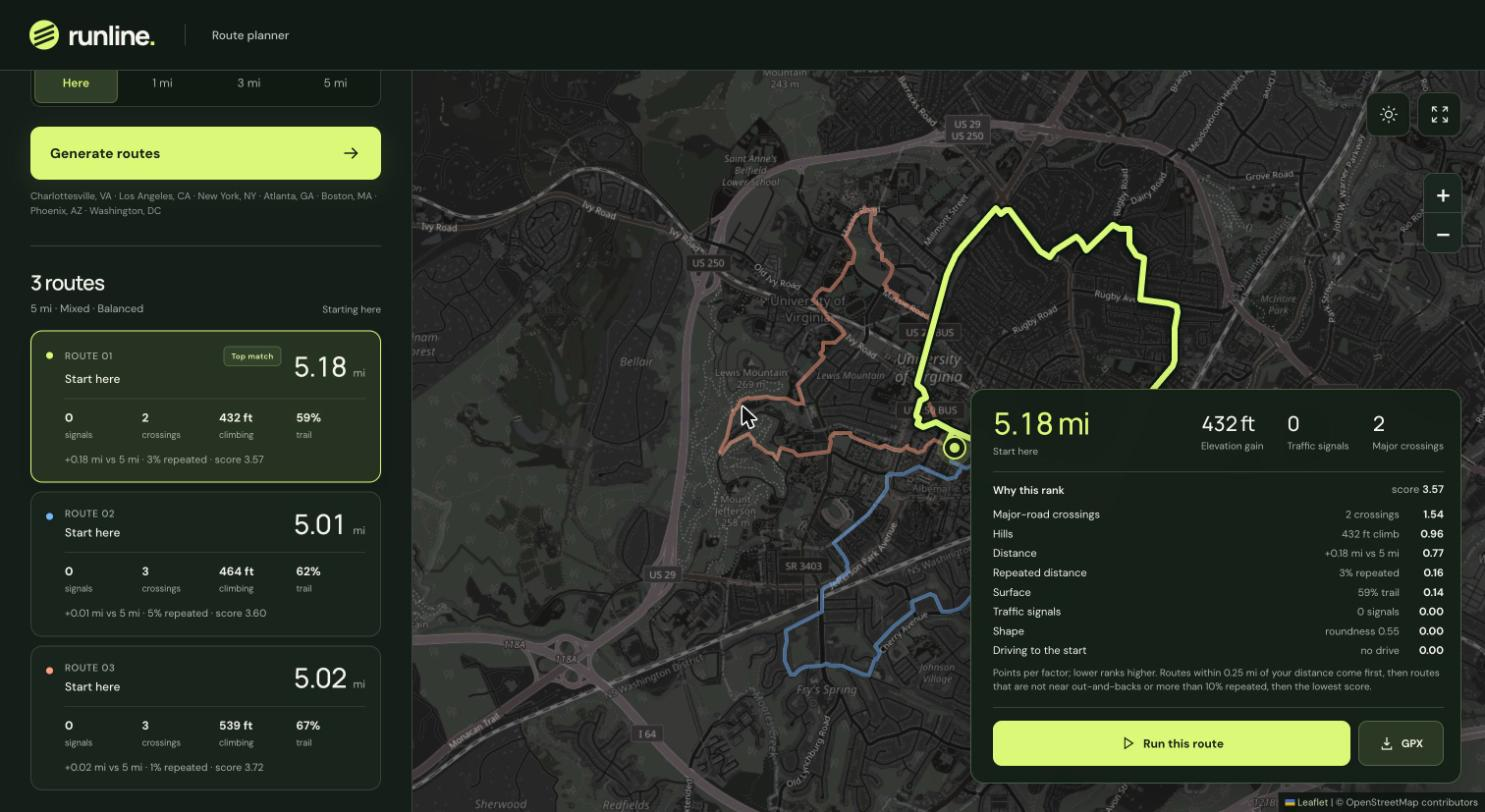
\includegraphics[width=\linewidth]{figures/app-results.jpg}
\caption{The deployed interface after a 5 mile request from the Rotunda
(18 November, after the fix). Each card shows crossings, distance off target,
repetition and score; the panel's ``Why this rank'' list gives every scoring
component's measurement and points.}
\label{fig:app}
\end{figure}

\paragraph{Nearby starts (US9).}
Ten Charlottesville cases across 1, 3 and 5 mile radii returned 19 routes
from alternative starts, and none lay outside the selected radius by road or
straight-line distance. On 16 November the interface named the alternative
start and said how many nearby starts were checked, but showed neither the
route's score nor the added driving distance, so the comparison US9 asks for
was not visible. Since the 18 November fix each alternative-start card shows
its driving distance and score, and the panel says how far to drive to the
start. The rerun repeated all ten cases with the same result (19 routes, none
outside the radius) and confirmed both values are displayed.
These requests always plan live and took a median of 15.2\,s (worst
24.0\,s). In 5 of the 19 routes the reported driving distance was
\emph{shorter} than the straight-line distance, because it is measured
between the nearest road-network points and leaves out the short legs onto
the network. A fix (\#33) adds those legs: over all 37,061 pairs of a public
park and a shipped start within 3 miles of it, the drive was below the
straight line in 380 pairs before and in none after.

\paragraph{Response time (US10).}
Table~\ref{tab:latency} gives end-to-end times measured from a laptop
through the public site. Warm 3 and 5 mile requests met the criterion easily
in every area: a median of 0.48\,s and a 95th percentile of 1.95\,s over 66
requests. The slowest warm request took 14.0\,s (Los Angeles). First requests
in an area were slower, because the server has to load that part of the map,
and two first requests (Boston and New York, both typed addresses that also
had to be geocoded) took over 20\,s. US10 covers warm requests only, so these
do not fail it, but a runner opening the app in a new city meets exactly this
case.

Almost all of a first request's time is spent loading one map tile into
memory. On the regional server, rebuilding the largest tile of the
Atlanta, Boston and Phoenix batch (263{,}000 nodes) from its file took 6--7\,s of the request; reading and
decompressing it took 0.6\,s. Two changes deployed on 14 November target this
(\#24, \#25). Loading pauses Python's garbage collector, which cut that tile's
load from 6.7 to 3.8\,s over two runs each. The page also asks the server to
load a start's tile as soon as the start is set, while the runner is still
choosing a distance. The deployment script requests routes directly and so
measures the cold case in Table~\ref{tab:latency}. In a separate check through
the public site on 14 November, we set a start in a tile no one had used,
waited six seconds as a runner choosing a distance would, and requested a
route: four such first requests (Boston, Phoenix, Los Angeles, New York) took
0.4--1.8\,s. Without pre-loading, first requests at eight other fresh starts
took 3.7--10.5\,s after the garbage-collector change. These are single
requests per area, so they show the mechanism works, not its typical
benefit.

\begin{table}[ht]
\centering\small
\caption{US10: production response times, 3 and 5 mile loops (seconds, end to end).}
\label{tab:latency}
\begin{tabular}{@{}l r r r r l@{}}
\toprule
Area & Warm $n$ & Median & p95 & First request (median / worst) & Pool / live \\
\midrule
Charlottesville & 30 & 0.46 & 0.77 & 0.45 / 3.9 & 29 / 1 \\
Washington, DC & 6 & 0.45 & 6.09 & 6.8 / 7.0 & 6 / 0 \\
New York & 6 & 0.89 & 2.02 & 18.3 / 20.3 & 2 / 4 \\
Los Angeles & 6 & 0.61 & 14.04 & 6.9 / 7.0 & 6 / 0 \\
Atlanta & 6 & 0.33 & 0.74 & 4.5 / 5.0 & 6 / 0 \\
Boston & 6 & 0.51 & 0.60 & 5.6 / 23.1 & 6 / 0 \\
Phoenix & 6 & 0.36 & 0.59 & 7.0 / 7.1 & 6 / 0 \\
\midrule
All areas & 66 & 0.48 & 1.95 & & \\
\bottomrule
\end{tabular}
\end{table}

\paragraph{Rerun after the 18 November release.}
We repeated the whole deployed check after redeploying the backend (174
requests). Charlottesville and Washington answered every request well inside
the criterion, and over all areas warm 3 and 5 mile requests had a median of
0.44\,s and a 95th percentile of 1.42\,s, both better than on 16 November, so
US10 is still met as the proposal defines it. Three metro results were worse,
all on the regional server, which the backend release does not change. One
warm Los Angeles request took 29.0\,s, which alone puts that area's own 95th
percentile above 20\,s. First requests in a new city took up to 125\,s (New
York, planned live because its precomputed routes missed). One Boston request
lost its connection before any answer, so Boston passed 11 of 12 requests;
the other five areas passed all of theirs, and US11 still holds. The regional
server needs the same first-request work listed in Table~\ref{tab:actions}.

\paragraph{Additional areas (US11).}
All six metro areas passed every smoke check: 72 requests at 3, 5 and 8 miles
from public landmarks returned 216 routes, every one closed, within the
$\pm$0.25 mile band, and with a GPX file matching its geometry point for
point. Between 34 and 36 of each area's 36 routes were within 5\% of the
target, and all were within 10\%. For all 378 loop routes collected across
the run, the score we recomputed from each route's metrics matched the API's
order. The browser half of US11 is covered by the team checklist.

\paragraph{Supporting evidence for US8.}
Scripts confirmed that place search returned suggestions for five public
names, that picking one moved the start, and that a typed address and a map
click at the same point produced identical routes. A start-to-finish request
in Charlottesville returned a correct 3.48 mile path in 1.7\,s. These checks
support US8 but do not replace the three-person checklist the proposal
specifies. That checklist (Appendix~\ref{app:checklists}) had not been
recorded when this report was compiled, so US8 remains pending.

\paragraph{A defect found by the validation tooling.}
Both of our own rehearsal scripts failed against the public site before
making a single route request, while passing against the backend directly.
The cause is the place-list endpoint: the hosting platform's cache returns
it Brotli-compressed even to clients that only accept gzip, which browsers
handle but ordinary HTTP libraries do not. Runners are unaffected, but any
non-browser client, including our monitoring, is. On 18 November the same
cache returned gzip to every client, including one that asked for no
compression. The public site's \texttt{/api} route forwards to the backend,
and the platform's cache for that forwarding stored the backend's
already-compressed answer for whichever client asked first; the backend's own
cache was correct. Turning off caching on the forwarding route (\#34) gave
each client its requested encoding on a preview deployment.

\paragraph{A weak live answer.}
One 3 mile request from a park start was answered live with three routes
that were all close to out-and-backs (roundness 0.13), two of them repeating
23\% of their length. Live planning uses the 10\% repetition limit only to
order routes, not to exclude them. On 16 November the interface did not show
repetition at all; since the 18 November fix each card shows the repeated
share. To see how often this happens we planned live from all 48 public park
starts at 3 and 5 miles: 12 of the 95 answers showed at least one such route,
and in none of them was a rounder route within twice the distance tolerance
left unshown, because ranking already puts every rounder in-band route first.
Excluding these routes would therefore only return fewer of them, so the fix
(\#32) adds a notice instead: ``No rounder loop of this length was found
from this start'', with the count when only some routes are affected.

\subsection{Findings outside the acceptance criteria}
\paragraph{Route shape.}
The criteria do not mention route shape, but a route can pass all of them and
still be unpleasant to run. Of the 96 live routes in the default run, 93 were
within the $\pm$0.25 mile band, 8 had a roundness below 0.2 (close to an
out-and-back), and 12 repeated more than 10\% of their length. The median
route repeated 2.2\%. Served routes were cleaner: all 95 were in band, 2 had
roundness below 0.2 and 4 repeated more than 10\%, because precomputed routes
that repeat too much are filtered out when they are generated. The separate
shape audit on the rebuilt graph found no route entering a dead end, but
three with a short revisit, up from none on the previous graph.

\paragraph{Precomputed route coverage.}
On the 600-request check against the deployed Charlottesville data,
precomputed routes answered 548 (91.3\%): 184 mixed, 181 road and 183 trail.
The other 52 were planned live, which took a median of about 1.4\,s on the
requests we timed, against 64\,ms from precomputed routes. All 52
came from 7 of the 40 starts. Two of those starts missed on every request. One
had its nearest map point on a four-node fragment disconnected from the
street network. The other had no good loop at all, and live planning did
poorly there too (38\% repeated distance). A fix that retries from the nearest
connected point and searches a wider ring of cells raised the rate to
582/600 (97.0\%) with identical results for the earlier hits. It is written
and tested (pull request \#15) but not yet deployed.

\paragraph{Privacy.}
Reviewing the code for what it stores, we found no database, account or
request history. We did find two log lines that record location. When
pre-loading a map fails, the API logs the runner's exact start coordinates,
and when a precomputed route is unusable it logs the 200\,m cell the request
fell in. Neither is stored by RunLine, but the hosting platforms keep logs.
Both lines now name the area instead (\#31), with tests that fail if a log
line contains a start's coordinates or cell.

\paragraph{Robustness of the precompute pipeline.}
Precomputing a batch of metro areas is itself a large test of the planner:
batch \texttt{b2} (Chicago, Miami and Houston) ran the loop generator for
every start cell of three metro areas, producing about 850{,}000 precomputed
pools. One of its 4{,}000 cluster tasks failed after
2\,h\,20\,min with ``longitude must be between $-$180 and 180'', and because the
merge only runs when every task succeeds, the whole batch was blocked. The
cause was a retry step: when a direction's best attempt was a loop only a few
metres long, the generator scaled its next attempt by the ratio of target to
measured length, which can exceed 1{,}000, and placed waypoints thousands of
kilometres away. We reproduced it with a test on a 5\,m block, where a
20 mile request placed a waypoint 12{,}432\,km out. The fix (\#26) caps the
rescale at four times the base radius; with it, the benchmark and shape audit
produced identical routes, so earlier batches remained valid. Rerunning the
failed task exposed a second gap: the rerun recorded a newer code commit, and
the merge correctly refused to mix commits. We added an explicit
\texttt{--allow-commit} option that accepts a named commit only after the
code between the two has been checked to compute the same pools, and records
both commits in the merged file (\#41). Batch \texttt{b2} then merged with
850{,}512 precomputed routes.

\paragraph{Map data.}
Rebuilding the Charlottesville graph to keep signalized crosswalks raised the
number of signal nodes from 131 to 569, and counted signal events on the
benchmark rose from 38 to 74. This is not a regression in routing. The old
graph had dropped the crosswalk signals during simplification, so earlier
signal counts were undercounts. Of the six other metro areas, Atlanta, Boston
and Phoenix were built after this fix; Washington, New York and Los Angeles
still use graphs built before it.
